\documentclass[DIV=13,fontsize=11pt]{scrartcl}
\usepackage[utf8]{inputenc}
\usepackage{hyperref}
\usepackage{amsmath}
\usepackage{amssymb}
\usepackage{graphicx}
\graphicspath{ {/Users/johannes/Documents/GitHub/DM2022-LinearTransformers/Article/images} }


\title{Replication of "Transformers are RNNs: Fast Autoregressive Transformers with Linear Attention"}
%\head{Titel ersetzen und Sub-Titel streichen.}
\author{Viet-Anh Do and Johannes Bergner}
\date{28.3.2022}

\begin{document}
\maketitle
\section{Introduction}
%Beschreiben sie mit ein paar Sätzen den Kontext der replizierten/reproduzierten Arbeit. Es werden höchstens drei bis vier Paragraphen erwartet. Sie sollen hinreichend erklären, was das das Problem ist, das der Artikel bearbeitet, warum es ein wichtiges Problem ist und das die Beiträge des replizierten/reproduzierten Artikel ist. Zitieren sie in diesem Abschnitt relevante wissenschaftliche Arbeiten. 

Transformers introduced by Vaswani et al. (2017) are the state-of-the-art in  tasks like language understanding and image processing.  However their quadratic memory complexity within the self-attention mechanism weakens the efficiency when dealing with long sequences.  
Consequently a number of so called \("X\)-\(former"\)- models have been proposed, that improve the original Transformer in terms of computational and memory efficiency.

Aside from other approaches, such as Performer (Choromanski et al., 2020), Linformer (Wang et al., 2020) and Big Bird (Zaheer et al., 2020) the authors of "Transformers are RNNs" developed a Linear Transformer (Katharopoulus et al., 2020) to show how the quadratic complexity \(O(N^2)\)  can be reduced to a linear complexity of \(O(N)\) without reducing the accuracy.

Standard Transformers use the folllowing attention matrix:

\begin{align}
    Attention(Q, K, V) {=} V {=} softmax \left(\frac {QK^T}{\sqrt{D_{k}}}\right) V,
\end{align}

with the queries Q \( \in \mathbb{R}^{N \times D_{k}}\),  keys K \(\in \mathbb{R}^{M \times D_{k}}\) and values V \( \in \mathbb{R}^{N \times D_{v}}\), where N and M represent the lenghts of queries and keys (or values) and \(D_{k}\) and \(D_{v}\) the dimensions of the keys (or queries) and values. The softmax function is applied rowwise to \(QK^T\).

Katharopoulus et al. (2020) simplify this attention mechanism by generalizing equation (1) and replacing the softmax with the kernel feature map \(\phi (x) {=} elu(x) +1\):

\begin{align}
    V_{i}' {=} \frac{\phi(Q_{i})^T \sum_{j=1}^{i} \phi(K_{j})V_{j}^T}{\phi(Q_{i})^T \sum_{j=1}^{i}\phi(K_{j})}
\end{align}

Because of that \(\sum_{j=1}^{i} \phi(K_{j})V_{j}^T\) and \(\sum_{j=1}^{i}\phi(K_{j})\) can be computed once and reused for every query, this leads to a linear time and memory complexity of \(O(N)\). Furthermore, by representing these cumulated sums as \(S_{i}\) and \(Z_{i}\), they can be seen as states of an RNN for causal attention and computed from \(S_{i-1}\) and \(Z_{i-1}\) in constant time.

By testing, the Linear Transformer of Katharopoulus et al. (2020) performed an image generation task based on the CIFAR-10 dataset over 4,000 times faster than the normal transformer with the same accuracy.  These results seem to be extraordinary, which is why the Linear Transformer has been recognized in further scientific research as well as the paper \textit{Transformers are RNNs} has been recited about 250 times in nearly two years. 

Indeed, Linear Transformers seem to overpower the original Transformer using long sequences. In this paper, we attempt to replicate the copy task of \textit{Transformers are RNNs} to investigate, whether Linear Transformer converges stably and scale linear with the sequence length. Furthermore, we want to find out at which sequence length a Linear Transformer is faster than a softmax-based Transformer.



% Was ist der Beitrag des replizierten Artikels?
% Welche Teile der Arbeit wurden für die Replikation ausgewählt? Begründen Sie die Auswahl. Warum wurden andere Teile der Arbeit nicht repliziert?
% Welche neuen Erkenntnisse erwarten Sie durch die geplante Reproduktion? Was steht davon nicht in dem replizierten Artikel?
% Was ist der Beitrag bzw. sind die Beiträge Ihres Artikels über die Reproduktion der ausgewählten Arbeit?

\section{Scope of reproducibility}
%Erklären sie die Behauptungen/Hypothesen/Experimente des Artikels, die sie für ihre Replikation/Reproduktion ausgewählt haben.
%Motivieren und begründen sie ihre Auswahl. 
%Es ist sinnvoll, wenn sie sich auf die Behauptung konzentrieren, die der Hauptbeitrag des Artikels ist.
%Um den Hauptbeitrag herauszufinden, versuchen sie den Artikel in ein bis zwei Sätzen zusammenzufassen, z.B.
%\begin{quote}
   % ``This paper introduces a new activation function X that outperforms a similar activation %function Y on tasks Z,V,W.''  oder 
    
   % ``Dieser Artikel führt eine neuartige Aktivierungsfunktion X ein, welche die ähnliche Aktivierungsfunktionen Y für die Aufgaben Z,W,V deutlich verbessert.''
%\end{quote}
%Stecken sie den Umfang ihrer Replikation/Reproduktion so klar wie möglich ab. 
%Die Behauptungen ihres Berichts sollten durch die Ergebnisse ihrer Experimente unterstützt oder widerlegt werden.
%Schauen sie sich zum Beispiel diese Beschreibung an:
%\begin{quote}
   % ``Contextual embedding models have shown strong performance on a number of tasks across NLP. We will run experiments evaluating two types of contextual embedding models on datasets X, Y, and Z.'' oder 
    
   % ``Für Contextual-Embedding-Modelle wurde nachgewiesen, dass die bei einer Vielzahl von Aufgaben aus einem breiten Spektrum natürlichen Sprachverarbeitung (NLP) eine hervorragende Leistung erbringen. Wir evaluieren experimentell zwei verschiedene Arten von Contextual-Embedding-Modellen auf den Datensätzen X, Y, Z.''    
%\end{quote}
%Der Umfang ist zu breit angelegt und es fehlt die Erwartung für ein klares Ergebnis.
%Schauen sie sich die nächste Beschreibung an:
%\begin{quote}
%``Finetuning pretrained BERT on SST-2 will have higher accuracy than an LSTM trained with GloVe embeddings.'' oder

%``Das Anpassen eines vortrainierten BERT-Modells für die SST-2-Aufgabe führt zu einer höheren Klassifikationsrate als ein LSTM-Modell, das für GloVe-Einbettungen trainiert wurde''
%\end{quote}
%Hier ist klarer was bei der Reproduktion/Replikation herauskommen kann. Diese Aussage könnte durch ihre Ergebnisse tatsächlich bestätigt oder widerlegt werden. 

Due to their linear complexity, Linear Transformers are said to be highly efficient when the sequence length increases. Katharopoulus et al. (2020) evaluate their Linear Transformer on image generation, automatic speech recognition and a copy task of numbers.

 In order to examine computational cost and convergence property with growing sequence length, a copy task of number sequences is favourable because it is easy to increase the sequence length and to evaluate the results. Furthermore, an example of a copy task is already given in the Julia package Transformers.jl. We will use this example as a benchmark, that represents the performance of the Transformer by Vaswani et al. (2017). Based on that, we are going to replace the softmax-based attention function by a linear attention function. Then we apply different sequence lengths and examine, if the Linear Transformer performs faster but with the same precision as the original Transformer especially with high sequence lenghts. 
All in all we focussing on the following claims:

\begin{itemize}
    \item Claim 1: Linear Transformers converge stably and reache the same performance as the original Transformer.
    \item Claim 2: Linear Transformer scale linear with the sequence length.
    \item Claim 3: Linear Transformer perform faster than softmax-based Transformer.
\end{itemize} \\

\\ \section{Methodology}

%In this section you explain your approach -- did you use the author's code, did you aim to re-implement the approach from the paper description? Summarize the resources (code, documentation, GPUs) that you used. 

\subsection{Model descriptions}
A minimalistic model was developed to determine the convergence properties and computational cost of linear transformers. The transformer which was introduced by Vaswani et al. (2017) has been chosen as our baseline in this experiment. Unlike this aforementioned model which utilized softmax attention, the authors shifted the feature map into the module attention, computed the dot product of key and value instead of key and query so that the attention matrix never be explicitly computed and thus decrease the complexity from \(O(N^2 max(D,M))\) to \(O(ND^2M)\), where \(N >\) \(D^2\) in practice. Our target is to determine, whether linear attention converges stable, scales linear with the sequence length and runs faster than the softmax attention for different sequence lengths.
%Beischreiben sie die Modelle, die im Originalartikel genutzt werden, einschließlich der Architektur, der Zielfunktion und der Parameter. 
%Describe the models used in the original paper, including the architecture, learning objective and the number of parameters.

\subsection{Data descriptions}
For this synthetic task, we use sequences of 10 different symbols separated by a dedicated separator symbol and with different lengths. These sequences are randomly generated at the beginning of the code.
%Beschreiben sie die Datenmengen die sie genutzt haben und wie sie sie bekommen haben. 
%Describe the datasets you used and how you obtained them. 

\subsection{Hyperparameters}
We have mostly adjusted the hyperparameters of the given model in Transformers.jl according to the original paper. The number of head per Transformer is 8, with a head size of 64, which leads to the size of the whole Transformer of 512. The sequence length will be varied from 8 to 64, whereas the learning rate will stay constantly at  \(10^{-3}\).  The batch size after being adjusted to fit the memory of our GPU will be kept at 8. We also maintain the number of training step at 3,000. We acknowledge that reducing the batch size could lead to a decreasing in precision at the end. However, our focus is to determine the performance particularly in respect to time complexity and therefore, it's not necessary to increase this parameter at the moment. 
%Beschreiben sie, wie sie Hyperparameter gesetzt haben. Welche Quellen haben sie für die konkreten Werte genutzt (z.B. den Forschungsartikel, Code oder sie hatten eine wohlbegründete Vermutung, educated guess).
%Describe how you set the hyperparameters and what the source was for their value (e.g. paper, code or your guess). 

\subsection{Implementation}
The programming language used in the replication task is Julia. Due to a restriction of time, we have mainly taken most of the code from the package Transformers.jl as a template for the implementation. Other packages were:
\begin{itemize}
    \item Flux: a library for machine learning functions for Julia
    \item CUDA: programming interface for working with NVIDIA CUDA GPUs using Julia
    \item Tullio: a flexible macro to calculate Einstein sums
    \item NNlib: a package that provides a library of functions useful for neural networks, such as softmax, sigmoid, batched multiplication, convolutions and pooling
    \item Plots: package to visualize data in Julia
\end{itemize} \\


\\ For the synthetic task, we use a modified version of copy task based on the experiment which was used by Kitaev et al.  (2020). As mentioned above in 3.1, what we do to implement linear attention is to replace the function attention of Transformers.jl with our own code called linattention, which has been translated from the original PyTorch code of the authors to Julia code. The original code requires in addition one more function called splitHeads to reshape the 3D tensor to 4D tensor, which we have also included in the script and which is shown below. 

\begin{tabular}{b}
\begin{verbatim}
function splitHeads(x, batch_size, head, depth)
    x = reshape(x, (batch_size, :, head, depth))
end
\end{verbatim}
\end{tabular} \\

\\ Moreover, as the authors used the activation function elu(x) + 1 in original paper instead of relu(x) as in the Transformers.jl, we also attempt to implement elu(x) + 1 (which was called nelu in our script and is shown below) into the code to make sure that the performances of each model do not affected by different conditions and therefore they are comparable. 

\begin{tabular}{b}
\begin{verbatim}
begin
    function oftf(x, y)
        oftype(float(x), y)
    end
    
    function nelu(x, α=1)
        ifelse(x ≥ 0, float(x)+1, @fastmath oftf(x, α) * (exp(x) - 1)+1)
    end
end
\end{verbatim}
\end{tabular} \\

\\ Also we have trimmed functions of the copy task of Transformers.jl that were only needed when using a softmax attention like  \(apply\)\(\textunderscore\)\(mask\) for the sake of simplification. Lastly, instead of using Kullback-Leibler divergence as loss function, we apply cross entropy to calculate the loss for the gradient descent as given in the original work.


%Beschreiben sie, ob sie vorhandenen Code oder eigenen Code genutzt haben.
%Stellen sie Links zum Code bereit und beschreiben sie welche Programmiersprachen und Pakete genutzt wurden.
%Ihr Github oder Gitlab-Reposititory sollte öffentlich sein. 
%Das Reposititory sollte klar dokumentiert werden. 
%Describe whether you use the existing code or write your own code, with the link to the code and which programming languages/packages were used. Note that the github repo you link to should be public and have a clear documentation.

\subsection{Experimental setup}
Firstly, 8 random batches as training data will be created. They will go through 4 layers of encoders as well as 4 layers of decoders. At the end, the loss can be computed for each iteration, so that we can monitor the improvement of loss over each iteration. Furthermore, we can also observe the execute time of each model after a certain amount of iteration. To do so, we use an Nvidia Quadro P4000 with 8 GB of memory. Finally, we create test data randomly and give it in the trained model. The model then has to replicate the given sequence of numbers.

The Authors claimed, that their model can perform much better than the other implementation of Transformer for very long sequences due to the linearity property. Therefore, two models will be trained with increasing sequence length to verify this statement, namely Transformer with softmax attention and Linear Transformer with linear attention. Also we double the length of symbol sequence after each run, beginning with 8, 16, 32 and 64. The run time as well as convergency was reported afterwards.

Towards the convergency, both model do not always converge within 3000 steps. It might be due to the the very small batch size, as reducing batch size can result in worser performance of optimizer. 

We implemented our code in a Pluto notebook and uploaded all our files in our GitHub repository \url{https://github.com/jbergner1/DM2022-LinearTransformers/}. In order to run our code we recomment reading the Read Me. 


%Erklären sie, wie sie ihre Experimente durchgeführt haben. Was für Ressourcen haben sie verwendet, z.B. GPU/CPU-Ressourcen.
%Verlinken sie ihren Code und Notebooks. 
%Explain how you ran your experiments, e.g. the CPU/GPU resources and provide the link to your code and notebooks. 

\subsection{Computational requirements}
Due to the linearity property as mentioned by the authors, we expect that the runtime of 3000 steps will just double after each run. We keep increasing the sequence length and keep other factors the same until the GPU reachs ist capacity. In this case, the maximal capacity can only be reached at \(seq\)\(\textunderscore\)\(len\) = 64. We also expected that Linear Transformer will perform better than Transformer with Softmax Attention in respect to computational time and convergency for long sequences.

%Beschreiben sie die Anforderungen für die Berechnungen für jedes ihrer Experimente, z.B. die Anzahl der CPU/GPU-Stunden oder die Voraussetzungen für den Hauptspeicher und GPU-Speicher. 
%Geben sie für Zeit und Speicher eigene Abschätzungen an, bevor die Experimente gelaufen sind und vergleichen sie dies mit den tatsächlich verbrauchten Ressourcen.
%Sie müssen vor den Experimenten einplanen, dass diese Informationen auch durch ihren Code gemessen und gespeichert werden.

% Provide information on computational requirements for each of your experiments. For example, the number of CPU/GPU hours and memory requirements.
% Mention both your estimation made before running the experiments (i.e. in the proposal) and the actual resources you used to reproducing the experiments. 
% \textbf{\textit{You'll need to think about this ahead of time, and write your code in a way that captures this information so you can later add it to this section.} }


\section{Results}
Due to the lack of memory capacity of the GPU, we can only set the sequence length to 64 at the maximum. 

\begin{table}[htbp]
\caption{Computational time of softmax and linear Transformer for given sequence lenghts}\\
\centering
\begin{tabular}{l c {4cm} l r {4cm} l z{4cm}|}
\multicolumn{3}{l}{\textbf{Computational time in seconds} }        \\ \hline \hline
Seq\_len      & Softmax      & Linear \\  \hline
8             & 221          & 1738   \\
16            & 236          & 3004   \\
32            & 287          & 5373   \\
64            & 416          & 10071  \\ \hline \hline
\end{tabular}
\end{table} \\

The result can be seen in table 1 (this table is presented as a plot in the Supplementary Material).

\\As mentioned, we can not implement higher sequences to empirically determine the point where Linear Attention outperforms Softmax Attention. To tackle this deficiency, we apply a R-code using regression to determine the sequence length, from which Linear Attention takes advantage over Softmax Attention. First, we assume that the computational time in case of Softmax Attention has quadratic relation and Linear Attention has linear relation to sequence length. We do a regression of time on sequence length to calculate the coefficients, then try to use this coefficients to predict the possible output. At the end, we set the two terms equally and solve the quadratic equation resulting from it.  A plot of that is shown in figure 1.

\begin{figure}[h]
    \centering
    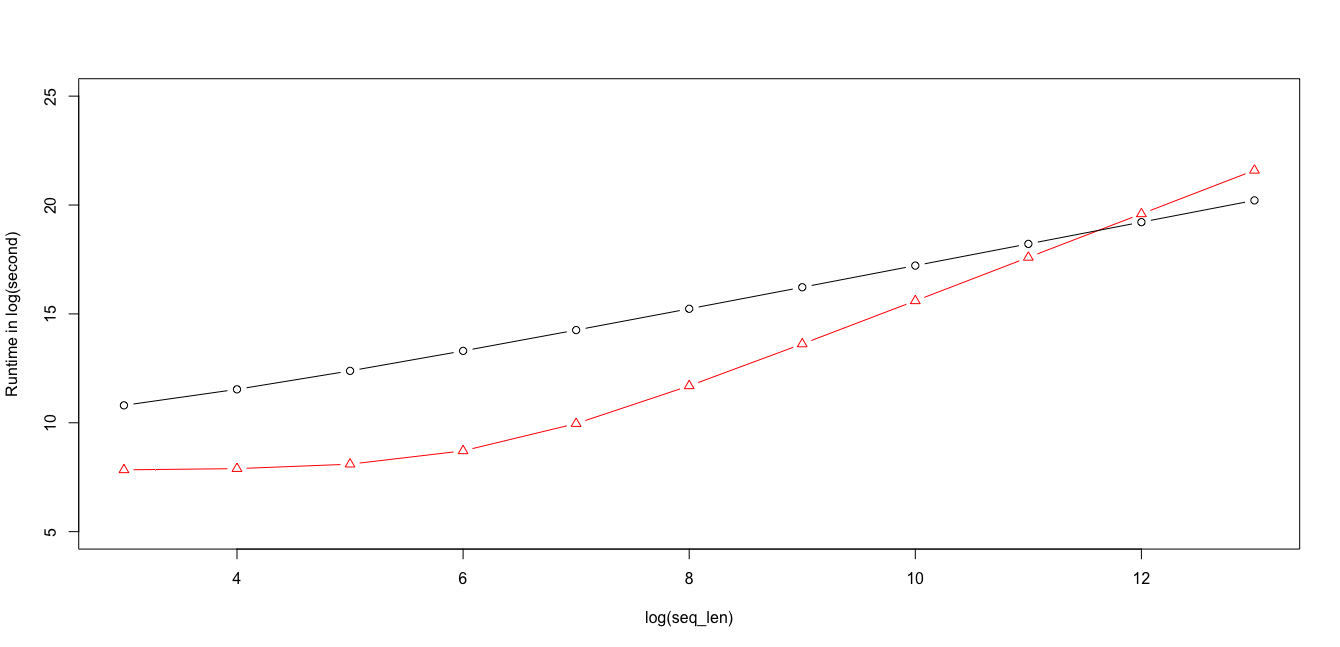
\includegraphics[width=\textwidth]{Rplot}
    \caption{Computational time and sequence length prediction based on R-Code}
    \label{fig:mesh1}
\end{figure}


%Starten sie mit einem Überblick über die Ergebnisse.
%Bestätigen ihre Ergebnisse die aufgeführten Behauptungen?
%Dieser Abschnitt sollte hauptsächlich Fakten nennen und so präzise wie möglich geschrieben werden.
%Die Bewertung und Diskussion kann im späteren Kapitel ``Diskussion'' folgen. 

% Start with a high-level overview of your results. Does your work support the claims you listed in section 2.1? Keep this section as factual and precise as possible, reserve your judgement and discussion points for the next ``Discussion'' section. 

%Beschreiben sie dann detailliert jedes einzelne Ergebnis, das sie haben.
%Zeigen sie wie es mit einer oder mehreren Behauptungen in Beziehung steht.
%Erklären sie konkret was der Kern ihres Ergebnis ist.
%Gruppieren sie die Ergebnisse in logische Abschnitte.
%Beschreiben sie klar, wo sie über den Originalartikel hinausgegangen sind, wo sie zusätzliche Experimente durchgeführt haben und wie diese mit den ursprünglichen Behauptungen in Beziehung stehen.

% Go into each individual result you have, say how it relates to one of the claims, and explain what your result is. Logically group related results into sections. Clearly state if you have gone beyond the original paper to run additional experiments and how they relate to the original claims. 

%Tipp 1: Drücken sie sich genau aus und verwenden sie eine klare und einfache Sprache, z.B. 
%\begin{quote}
 %   ``we reproduced the accuracy to within 1\% of reported value, that upholds the paper's conclusion that it performs much better than baselines.'' oder

    %``We konnten die Klassifikationsrate bis auf 1\% des angegebenen Werts reproduzieren. Dies unterstützt die Schlussfolgerung der Artikels, dass der Ansatz leistungsfähiger als die Baselines ist.''
%\end{quote}
%Oft kann man nicht die exakt gleiche numerische Zahl als Ergebnis bekommen. Deshalb müssen sie das Ergebnis bewerten, um zu entscheiden, ob ihr Ergebnis die Behauptung der Originalartikels unterstützt.
% Getting exactly the same number is in most cases infeasible, so you'll need to use your judgement call to decide if your results support the original claim of the paper. 

%Tipp 2: Nutzen sie Tabellen und Abbildungen, um ihre Ergebnisse darzustellen. 
% You may want to use tables and figures to demonstrate your results.

% The number of subsections for results should be the same as the number of hypotheses you are trying to verify.

\subsection{Result 1}
Katharopoulos et al. (2020) claim, that their Linear Transformer converges stable and reaches the same performance level as the original Transformer.  Figure 2 shows the Convergence Plots of the Linear Transformer. Looking at these plots, a stable convergence does not occur.  Even though the Linear Transformer converges to 0 at a sequence length of 8 and 32, the original Transformer converges to a loss that ranges from 10 to 18, whereas the Linear Transformer converges from 0 up to 70.  

The original convergence plot of  \textit{Transformers are RNNs} contains 10,000 gradient steps. We could just analyze 3,000 steps, but looking at the original plot of the paper, linear attention has a higher loss than softmax attention on that point. Nevertheless, the original plot shows a range of the loss between \(10^{-2}\) and  \(10^{-1}\).  This is something we can not replicate with our small  batch size and number of gradient steps.

Consequently the Linear Transformer has much more variation in its losses and does not converge stably. 

\begin{figure}[h]
    \centering
    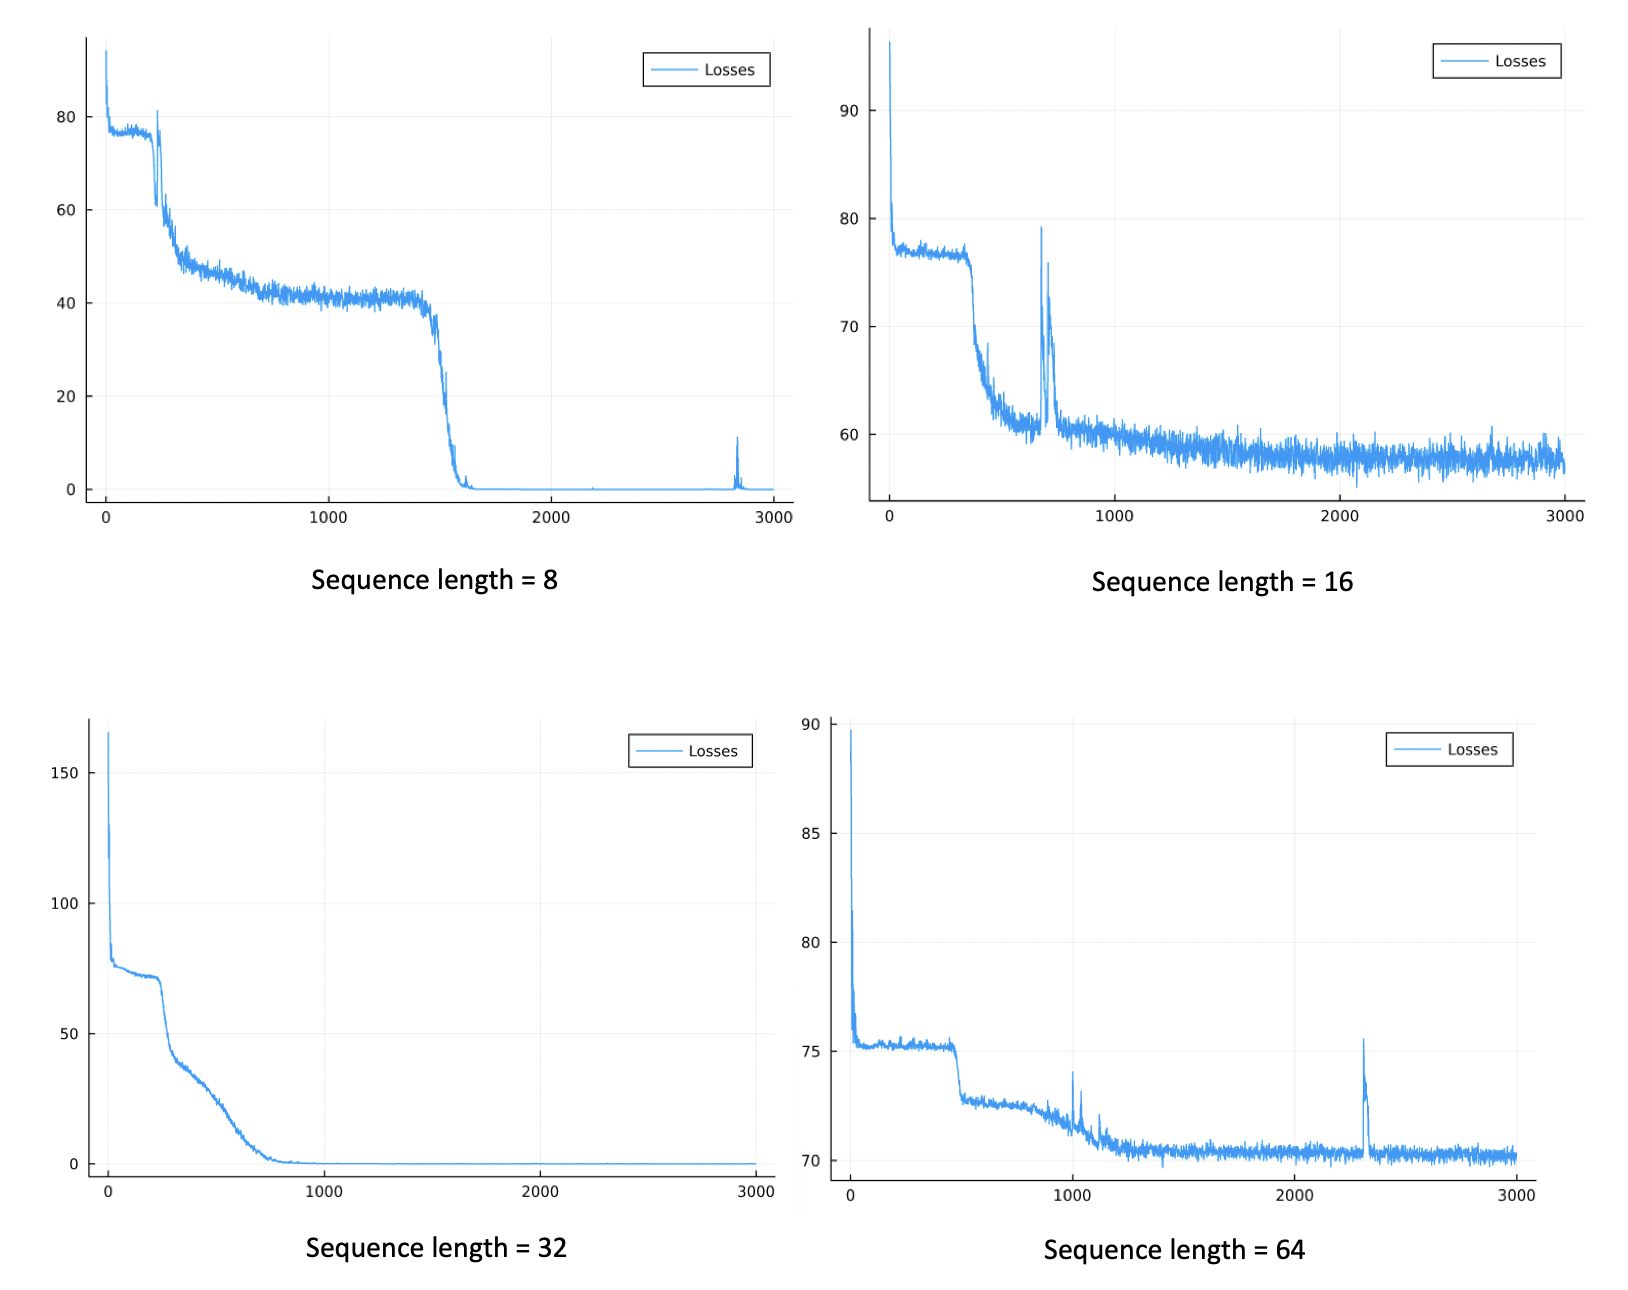
\includegraphics[width=\textwidth]{conv_plot_linear}
    \caption{Convergence Plots of Linear Transformer with 3,000 gradient steps}
    \label{fig:mesh1}
\end{figure}

\subsection{Result 2}
Like its name says, a Linear Transformer is supposed to scale linear to the sequence length. Our findings confirm this. Looking into table 1, each doubling of the sequence length approximately
doubles the computational time of the Linear Transformer. So we were able to implement a linear complexity to the basic Transformer of Transformers.jl. 
Figure 1 also shows, that the Linear Transformer scales linear with the sequence length, whereas the softmax-based Transformer shows signs of quadratic complexity.


\subsection{Result 3}
Katharopoulos et al. (2020) often claim, that the Linear Transformer is faster than a softmax-based Transformer as a general statement. They analyze sequence lenghts of of \(2^9\) or higher and confirm that statement. 

In contrast to \textit{Transformers are RNNs} we analyzed smaler sequence lengths beginning at  \(2^3\) and ending at \(2^6\).  As we expected, Softmax Attention does overperform Linear Attention by short sequences up to the length of \(2^6\). This result shows, that linear attention performs only well with long sequences.  So softmax attention is still advantageous on short sequences.

As a matter of fact that the capacity of our GPU was relatively restricted and that the code could have been implemented more efficiently,  we cannot experiment with a higher sequence lengh to determine empirically the point where linear attention begins to outperform softmax attention.  Because of that, we calculated the relationship between runtime and sequence length in R with our experimental data as the basis. According to the calculation, it is only worthwhile to use Linear Attention from a sequence length of 3149, i. e.  between \(2^{11}\) and \(2^{12}\). This result is not inline with the experiment in the original article, which claims that the outperformance of linear attention should already occur from a sequence length of \(2^9\) = 512. 
%Beschreiben sie alle zusätzlichen Experimente, die über den Originalartikel hinausgehen.
%Dies können Experimente zu weiteren Datenmengen sein oder sie probieren andere Methoden bzw. weitere Vereinfachungen des Modells aus oder passen die Hyperparameter an.
%Beschreiben sie für jedes zusätzliche Experiment, was sie genau durchgeführt haben, was die Ergebnisse sind und diskutieren sie was diese Ergebnisse zeigen. 

% Describe any additional experiments beyond the original paper. This could include experimenting with additional datasets, exploring different methods, running more ablations, or tuning the hyperparameters. For each additional experiment, clearly describe which experiment you conducted, its result, and discussions (e.g. what is the indication of the result).

\section{Discussion}
Our experiments show, that Linear Transformer are faster than softmax-based Transformer with a quadratic complexity, but only when using long sequences. Katharopoulos et al. (2020) explain the problems of the original Transformer with growing sequence lenghts and provide their Linear Transformer as a solution. In this regard they claim, that linear attention performs faster than softmax attention. Our replication finds, that this is only true with long sequences and not as a general statement. So as a consequence, the original Transformer is still more useful, when the sequences are small. 

With our implementation, we were able to linearize the complexity of a Transformer to the sequence length. This shows that the mathemetical trick that Katharopoulos et al. (2020) explain works and delivers results. 

Nevertheless, we could not replicate a stable convergence of the Linear Transformer. Looking at Figure 2 our implementation of a Linear Transformer always converges with several steps. This is comparable to the convergence of the original Transformer. As we look at Figure 3, the convergence plots seem quite similar (apart from the Linear Transformer having a higher loss).

\begin{figure}[h]
    \centering
    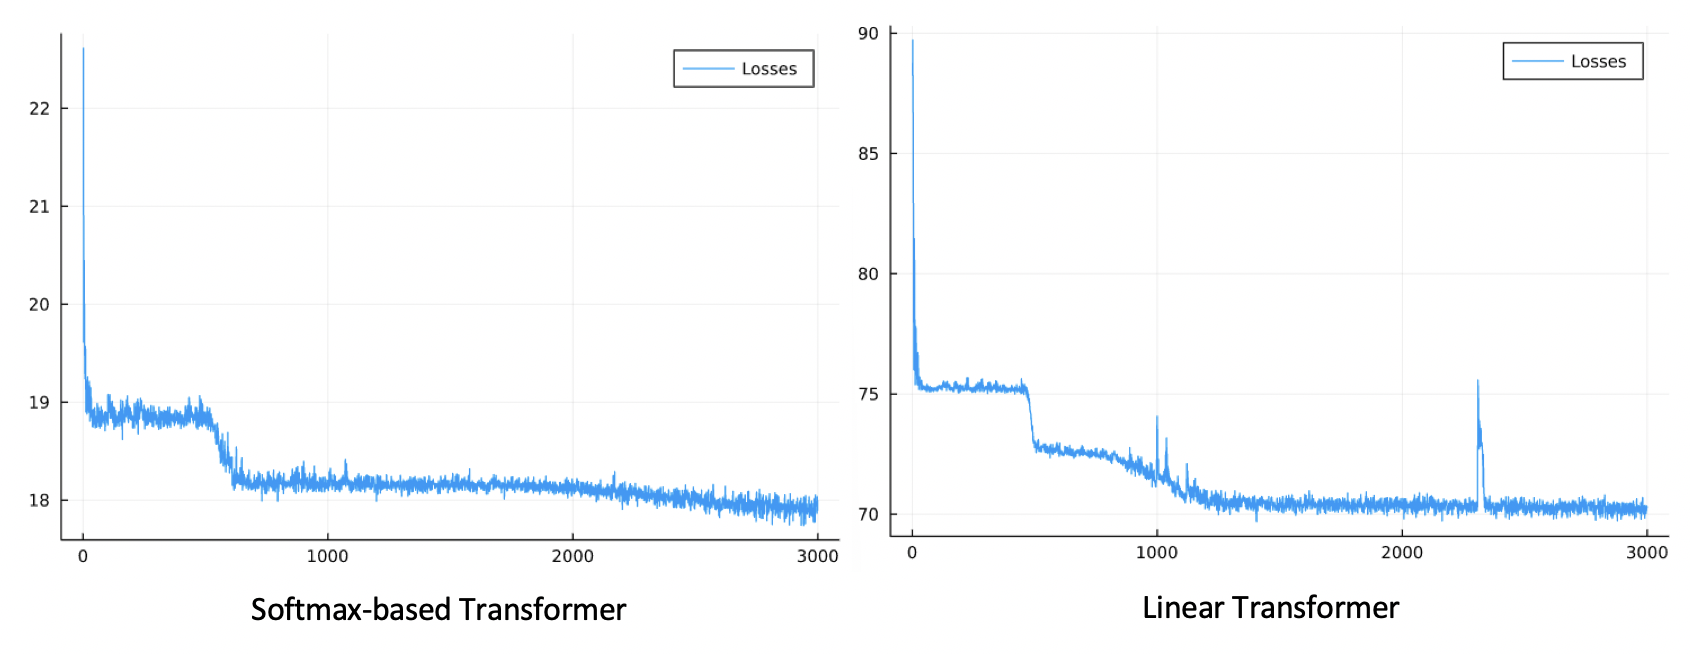
\includegraphics[width=\textwidth]{comparison}
    \caption{Convergence Plots of Original and Linear Transformer with 3,000 gradient steps and a Sequence length of 64}
    \label{fig:mesh1}
\end{figure}

In Summary, we can conclude, that we were partly able to replicate the findings of  \textit{Transformers are RNNs} in our implementation of a Linear Transformer using Julia. We developed a Transformer that scales linear to the sequence length, just like proposed in the paper. However, we could not discover a stable convergence of the Linear Transformer and our Transformer overpowers a softmax-based Transformer only above a sequence length of \(2^{12}\),  whereas the paper proposed this happens already at \(2^{9}\). 

Reasons for the failure of the replication could also be linked to our implementation itself. Our code in Julia could be further optimized and implemented more effiziently. Whereas the authors use PyTorch as a Python library with many functions for specific machine learning tasks, we had to either find equivalents in Julia or implement these functionalities ourself. This may sometimes resulted in a way that worked for our use case, but did the computation not in the best way. The code implementation of a Linear Transformer by Katharopoulos et al. (2020) differed in certain parts from the explanation of the paper. They used for example Einstein summation to compute the matrices more efficiently and some calculations were written in C++ in order to optimize them. Since we used plain Julia, this could be one reason for the underperformance of our Linear Transformer in comparison to the original. 

In the GitHub repository of \textit{Transformers are RNNs} it is rather described, how the repository can be used as a package in order to apply the Linear Transformer. On the other hand, it is a little bit unclear, how the Transformer was optimized and which function is necessary to implement it efficiently. Whereas the paper describes the proposed Transformer very detailled, the code implementation of it has quite a lack of explanation.  So we can not be exactly sure whether our implementation uses the most efficient calculations.

% Describe larger implications of the experimental results, whether the original paper was reproducible, and if it wasn’t, what factors made it irreproducible. 
The advantage of our approach was, that we could analyze different sequence lengths by modifying the amout of numbers on our copy task. Because of that we could create new findings in a fast way without many changes in the code. We mainly had to change the attention function of the Transformer provided by the package Transformers.jl. Therefore it was easy to change the existing softmax-based Transformer into a Linear Transformer.

Unfortunately we could not analyze sequence lengths above \(2^6\) because of limited GPU memory. Maybe with an optimized version of our Transformer, running with longer sequences would be possible. 

We used a Transformer as our basis, which usually has a softmax attention. and is probably optimized for it. Maybe our result would be closer to the ones of \textit{Transformers are RNNs} if we develop a Transformer that is basically planned to use linear attention. E.g. we had to reshape the structure of matrices in order to fit the requirements of our basic Transformer from Transformers.jl. This takes computation time, which could be lowered by implementing a Transformer that is more suitable for linear attention.

In our replication we only focused on the a copy task to compare linear and softmax attention. The paper also views the tasks image generation and automatic speech recognition. Maybe these tasks would have shown the differences between the original and the Linear Transformer more clearly and highlighted the strengths of the linear attention. 
%Diskutieren sie die Stärken und Schwächen ihres Ansatzes, vielleicht haben sie aus Zeitgründen nicht alle Experimente durchführen können, oder vielleicht haben zusätzliche Experimente durchgeführt, die den Originalartikel weiter stärken. 
All in all, we believe that the claims by Katharopoulos et al. (2020) are true and solve the problem of softmax attention with growing sequence length. Although our Linear Transformer did not perform as efficient as the one from the paper, we think that with further optimization it is possible to achive similar results.
% Give your judgement on if you feel the evidence you got from running the code supports the claims of the paper. Discuss the strengths and weaknesses of your approach -- perhaps you didn't have time to run all the experiments, or perhaps you did additional experiments that further strengthened the claims in the paper.

\subsection{What was easy?}
Katharopoulos et al. (2020) describe the mathematical simplification on order to achieve a linear complexity very detailed and justify each point understandable. So with an intermediate knowledge of matrix calculation and Transformers in general, the idea of the paper is perspicuous. This is supported by slides and videos of lectures about Linear Transformers which the authors provide on their website. 

Furthermore Katharopoulos et al. (2020) provide code to their Linear Transformer on GitHub. This repository is usable as a PyTorch package to apply Linear Transformers without an own implementation. Because of that, the GitHub repository is very extensive and contains useful information. The authors also refer to other repositories which use PyTorch as well as TensorFlow to implement a Linear Transformer. This wide number of templates was useful to create our own version of a Linear Transformer in Julia. Additionally the package Transformers.jl exists in Julia. It already contains an implementation of a softmax-based Transformer introduced by Vaswani et al. (2017). Moreover Transformers.jl had an example of a copy task which we used as the basis of our implementation. With an understanding of the tasks done in the paper and the code templates in Python it was possible for us to analyse the code of the copy task of Transformers.jl and mark sections, where changes are needed. Consequently, we changed the softmax-based attention function into a linear attention function. The rest of the example only needed minor changes in order to run our Linear Transformer.

At first we tried to run our code on a CPU, which resulted in a long time to carry out the experiments. Fortunately we were able to use the server provided by our University in order to run the code on a GPU. Because of that we could run code on several computers and procured results fast and effectively. 


%Beschreiben sie welche Teile der Replikation/Reproduktion sich leicht umsetzen ließen.
%Lief der Code der Autoren problemlos? War es aufgrund der Beschreibung im Originalartikel nicht aufwändig die Methoden zu reimplementieren? 
%Dieser Abschnitt soll den Lesenden zeigen, welche Teile des Originalartikels sich leicht für eigene Ansätze verwenden lässt. 

% Describe which parts of your reproduction study were easy. E.g. was it easy to run the author's code, or easy to re-implement their method based on the description in the paper. The goal of this section is to summarize to the reader which parts of the original paper they could easily apply to their problem. 

%Tipp: Machen sie keine pauschalen Verallgemeinerungen. Was für sie leicht ist, muss für andere nicht leicht sein. Geben sie genügend Kontext und erklären sie warum manche Sachen leicht waren, z.B. der Code hatte eine umfangreiche Dokumentation der Schnittstellen und viele Beispiele aus der Dokumentation passten zu den Experimenten im Artikel. 

% Be careful not to give sweeping generalizations. Something that is easy for you might be difficult to others. Put what was easy in context and explain why it was easy (e.g. code had extensive API documentation and a lot of examples that matched experiments in papers). 

\subsection{What was difficult?}
The paper Transformers are RNNs seemed to support an implementation of Linear Transformers, because it contains an algorithm that explains how the calculation can be done using for-loops. However, the code differs from this algorithm. Instead of for-loops, Katharopoulos et al. (2020) use Einstein sums for calculation, which are never mentioned in the paper. With no knowledge of that specific mathematical operation it was challenging to discover how the matrices are computed. This was also caused by the reason, that the authors used the package torch to implement Einstein summation. This package does not exist in Julia, so we had to find a package that does the same calculation. For that we had to do further research in the computational function of Einstein summation and compare the one of torch with equivalent Julia packages. Lastly, after a consultation with our lecturer, we decided to use the package Tullio.jl. In addition to that, torch used another syntax to specify the input and the required transformation of the matrices. Consequently we needed to find a translation from the torch syntax to the one used in Tullio.

In general, it was a challenge to translate the code templates written in Python into Julia since Julia does not use classes like object-oriented languages. It was e.g. not possible to access values of a class, so we had to pass values within functions. Because of that, the code written in Julia is different than the Python template in some cases. Furthermore, many codes contained reshapes of the matrices, but did not mention which structure resulted from it. We had a lot of problems because of wrong matrix shapes, which were laborious to solve.  We had e.g. to reference from other code source to find solutions.

Katharopoulos et al. (2020) published their experiments in a separate repository on GitHub, which is only mentioned in the issues section. There is no reference to this repository in the ReadMe, but on the other hand other references lead to non-existing pages that show a 404-error. In the repository, which can be used as a package, calculations are partially written C++. Because of that, the code published by the authors was all in all hard to understand. 

We also ran the copy task provided in the experiment repository of Katharopoulos et al. (2020). Unfortunately, this code showed only the loss and accuracy of the model during the training, but did not give a plot or overview of the loss in the end. Furthermore, the ReadMe did not specify, how sequences of numbers can be applied in order to test the model. Finally, we were not able to generate any findings from the provided code.

In order to use our Linear Transformer written in Julia on a GPU, we had to use CUDA. This package requires a Nvidia graphic card, which we could only access by using the University-servers. These servers did not always run stably, so that some experiments needed to be run again. The problem of using external servers to have a Nvidia GPU is an issue that may also affect multiple users.

At last but not the least, we wrote to the authors about our problems and questions, but have not received an answer yet. Looking at the issues section on the GitHub repository, it sometimes takes months to receive any responses from the authors.


%Beschreiben sie welche Teile ihrer Replikation/Reproduktion aufwändig oder schwierig waren oder viel mehr Zeit in Anspruch genommen haben, als sie erwarteten.
%Vielleicht waren Daten nicht verfügbar, so dass sie einige Experimente nicht verifizieren konnten, oder der Code der Autoren funktionierte nicht und musste erst debugged werden.
%Vielleicht dauerten auch einige Experimente zu lange und sie konnten sie deshalb nicht verifizieren.
%Dieser Abschnitt soll den Lesenden zeigen, welche Teile des Originalartikels schwer wiederverwendbar sind, bzw. signifikante Zusatzarbeiten und Ressourcen erfordern. 

% Describe which parts of your reproduction study were difficult or took much more time than you expected. Perhaps the data was not available and you couldn't verify some experiments, or the author's code was broken and had to be debugged first. Or, perhaps some experiments just take too much time/resources to run and you couldn't verify them. The purpose of this section is to indicate to the reader which parts of the original paper are either difficult to re-use, or require a significant amount of work and resources to verify. 

%Tipp: Setzen sie sorgfältig ihre Diskussion in den richtigen Kontext, z.B. sagen sie nicht `` die Mathematik war schwer verständlich'' sondern sagen sie `` die Mathematik erfordert fortgeschrittene Kenntnisse in Analysis für das Verständnis''.

% Be careful to put your discussion in context. For example, don't say ``the math was difficult to follow,'' say ``the math requires advanced knowledge of calculus to follow.'' 

\subsection{Recommendations for reproducibility}
In order to improve the replicability, Katharopoulos et al. (2020) should add comments to their code. Thereby it will be possible to explain the structure caused by the reshape of matrices and requirements of certain functions, which depends on the shape of a matrix. Furthermore,  it should have been shown, which part of the paper is implemented in a certain line of code and why e.g. a package is used to do a calculation.

Although the authors answer question in the issues section in GitHub very well, they should add these answeres to their repository to prevent, that these questions occur again. In our case it was always more useful to search in the issues section than in the ReadMe of the repository when we had questions.
%Geben sie Empfehlungen, wie die Autoren des Originalartikels oder andere Forschende in diesem Feld die Replizierbarkeit / Reproduzierbarkeit verbessern können.

% Describe a set of recommendations to the original authors or others who work in this area for improving reproducibility.

\section{Communication with original authors}
Our contact to the authors was unanswered. However, the issues section in the GitHub Repository contains questions that are also interesting in our case.

The user gaceladri made his own implementation of a Linear Transformer and shared a plot that showed, that the loss of a Linear Transformer is higher than the loss of a softmax-based Transformer (in this case a BERT model) when the gradient steps are lower than 10,000.  The user asked, if he has done something wrong regarding this discovery. Angelos Katharopoulos (username: angeloskath) answered, that this is possible, because the attention matrix of a Linear Transformer is low rank which leads to a harder learning process. The author further explains, that the whole point of Linear Transformers is an optimization of speed and memory. When these aspects are insignificant, using a softmax attention is probably better. 

The user Yogurt928 asked, why Einstein sums are used in the code, whereas the paper uses buzz signs. Katharopoulos responds: 
\begin{quote}
"The reason for using einsum instead of multiplication and summation is that it is faster since the large matrix does not need to ever be computed and kept in memory."
\end{quote}

At last, the user burcehan asked, why \(elu(x) + 1\) was used as the feature map.  He recognized, that the convergence of his model is very slow using this function.
Angelos Katharopoulos answers that the feature map needs to correspond to a non-negative similarity score. The question, whether other feature maps are better is an open research problem. In the tests for the paper, some feature maps achieved similar results, others not. All in all this depends on the analysed problem, but problems that require sparse attention patterns might be harder to learn using the \(elu(x) + 1\) feature map.

%Dokumentieren sie das Ausmaß (oder das Fehlen) der Kommunikation mit Autoren.
%Stellen sie sicher, dass der Bericht eine faire Beurteilung der Forschungsarbeiten ist. Versuchen sie deshalb mit den Autoren Kontakt aufzunehmen.
%Sie können ihnen konkrete Fragen stellen oder falls sie keine Fragen haben, den Bericht zusenden und um Feedback bitten.



% Document the extent of (or lack of) communication with the original authors. To make sure the reproducibility report is a fair assessment of the original research we recommend getting in touch with the original authors. You can ask authors specific questions, or if you don't have any questions you can send them the full report to get their feedback.



% \section{Lösungsansätze für das Problem}
% Kurze Zusammenfassung verwandter/konkurrierender Arbeiten, die das Problem auf ähnliche Weise lösen (zwei Artikel oder mehr)
% Erste Gruppe von Artikeln 
% Zweite Gruppe von Artikeln
% Kurze Zusammenfassung von Arbeiten, Methoden oder Techniken auf denen der replizierte Artikel aufbaut (zwei Artikel oder mehr)
% Erste Gruppe von Artikeln 
% Zweite Gruppe von Artikeln 
% Kurze Beschreibung des/der Ansatzes/Ansätze, die für die Replikation ausgewählt wurden.
% Offene Details, die im replizierten Artikel nicht oder unvollständig beschrieben wurden und die nicht zitierten Artikeln geklärt werden.
% Welche Details können durch die Reproduktion geklärt und ergänzt werden? Erklären Sie diese Details.
% Welche Prinzipien, Ideen, Grundlagen oder Annahmen stehen hinter dem replizierten Ansatz?



% \section{Empirische Evaluation und Replikation}
% Beschreibung der Implementierung 
% Beschreibung von einfachen Tests, die die Korrektheit der Implementierung belegen
% Beschreibung des Speicherverbrauchs und der Laufzeit-Performance der Implementierung
% Beschreibung der Ausgangsdaten
% Beschreibung der Vorverarbeitung der Daten
% Beschreibung der Replikation des/der Experiment/e
% Beschreibung von Schwierigkeiten und Problemen


% \section{Zusammenfassung}
% Ist der Ansatz gut genug, um das Problem als gelöst zu betrachten?
% Welche Schwierigkeiten des Ansatzes deckte die Replikation auf?
% Welche Forschungenrichtungen halten Sie für künftige Untersuchen für potentiell wichtig?

% \section{Entwicklung und Julia-Code}
% Implementierung Datenvorverarbeitung 
% Implementierung Modell
% Implementierung von Tests, Ausgaben, Grafiken, die Arbeitsweise und Korrektheit belegen
% Implementierung zur Auswertung offener Details im replizierten Artikel
% Implementierung des replizierten Experiments, Evaluation
% Implementierung Evaluationsauswertung


\newpage
\begin{thebibliography}{9}
\bibitem [Choromanski et al., 2021] {Choromanski} Choromanski, K., Likhosherstov, V., Dohan, D., Song, X., Gane, A., Sarlos, T., Hawkins, P., Davis, J., Mohiuddin, A., Kaiser, L., Belanger, D., Colwell, L., & Weller, A. (2021). Rethinking Attention with Performers. arXiv:2009.14794 [cs, stat]. http://arxiv.org/abs/2009.14794
\bibitem [Katharopoulos et al., 2020] {Katharopoulos} Katharopoulos, A., Vyas, A., Pappas, N., & Fleuret, F. (2020). Transformers are RNNs: Fast Autoregressive Transformers with Linear Attention. arXiv:2006.16236 [cs, stat]. http://arxiv.org/abs/2006.16236
\bibitem [Kitaev et al., 2020]{Kitaev et al., 2020} Kitaev, N., Kaiser, Ł., & Levskaya, A. (2020). Reformer: The Efficient Transformer. arXiv:2001.04451 [cs, stat]. http://arxiv.org/abs/2001.04451
\bibitem [Tay et al., 2020]{Tay} Tay, Y., Dehghani, M., Abnar, S., Shen, Y., Bahri, D., Pham, P., Rao, J., Yang, L., Ruder, S., & Metzler, D. (2020). Long Range Arena: A Benchmark for Efficient Transformers. arXiv:2011.04006 [cs]. http://arxiv.org/abs/2011.04006
\bibitem [Vaswani et al., 2017]{Vaswani}Vaswani, A., Shazeer, N., Parmar, N., Uszkoreit, J., Jones, L., Gomez, A. N., Kaiser, L., & Polosukhin, I. (2017). Attention Is All You Need. arXiv:1706.03762 [cs]. http://arxiv.org/abs/1706.03762
\bibitem [Wang et al., 2020]{(Wang et al., 2020} Wang, S., Li, B. Z., Khabsa, M., Fang, H., & Ma, H. (2020). Linformer: Self-Attention with Linear Complexity. arXiv:2006.04768 [cs, stat]. http://arxiv.org/abs/2006.04768
\bibitem [Zaheer et al., 2021]{Zaheer et al., 2021} Zaheer, M., Guruganesh, G., Dubey, A., Ainslie, J., Alberti, C., Ontanon, S., Pham, P., Ravula, A., Wang, Q., Yang, L., & Ahmed, A. (2021). Big Bird: Transformers for Longer Sequences. arXiv:2007.14062 [cs, stat]. http://arxiv.org/abs/2007.14062

\newpage
\section*{Supplementary Material}

\section*{Computational time over gradient steps}

\begin{figure}[h]
    \centering
    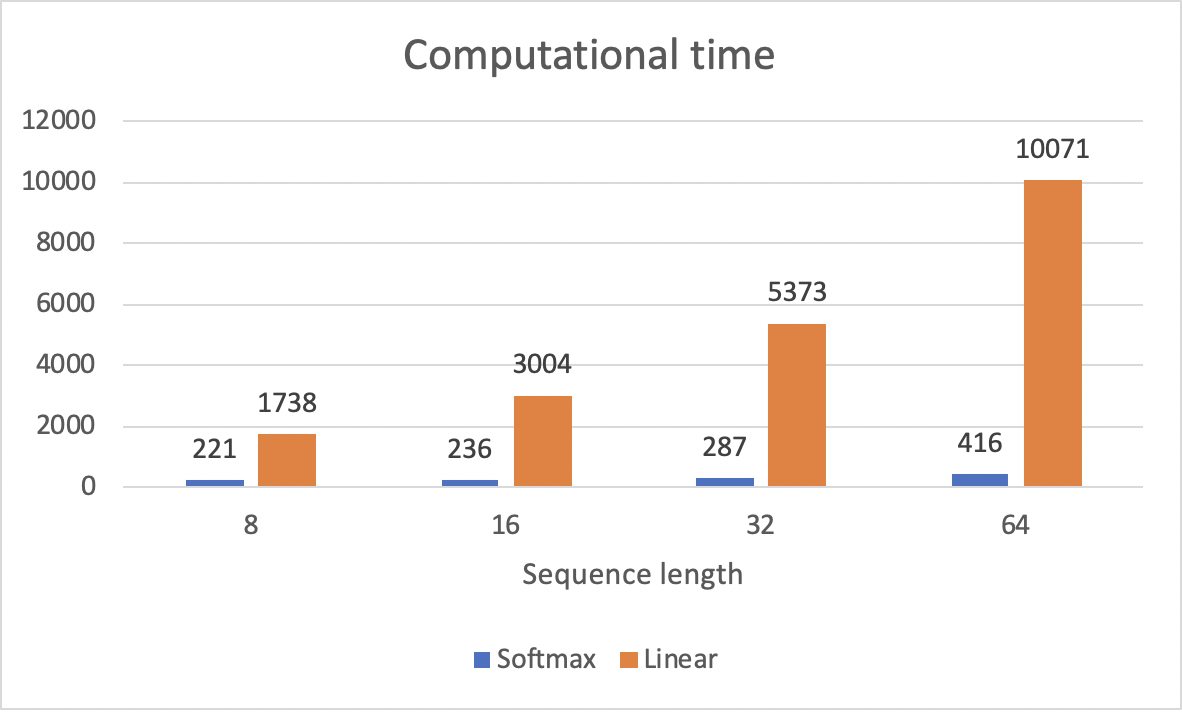
\includegraphics[width=\textwidth]{compTime_plot}
    \caption{Computational time of softmax and linear attention over 3,000 gradient steps}
    \label{fig:mesh1}
\end{figure}

\newpage
\section*{Convergence Plot of Softmax Transformer}


\begin{figure}[h]
    \centering
    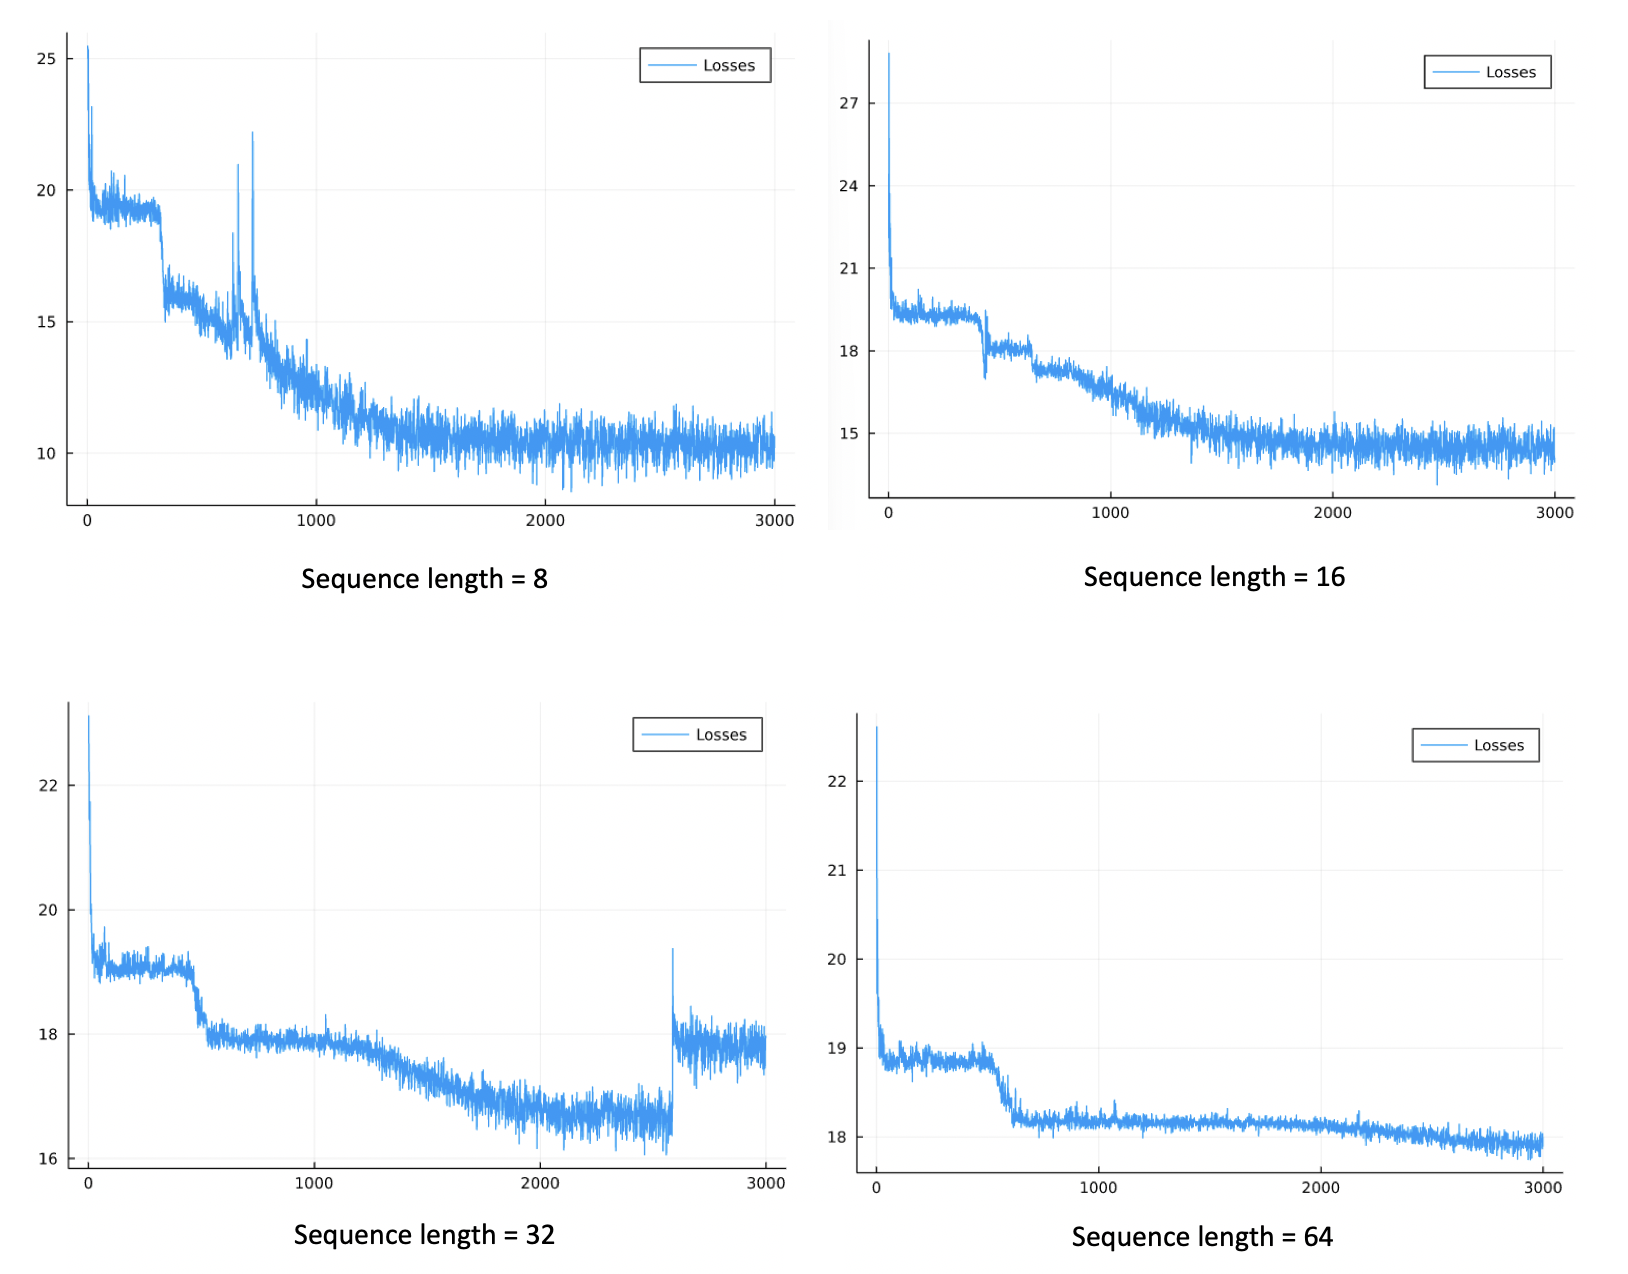
\includegraphics[width=\textwidth]{conv_plot_softmax}
    \caption{Convergence Plots of Softmax Transformer at 3,000 gradient steps}
    \label{fig:mesh1}
\end{figure}

\newpage
\section*{Git History}

\begin{figure}[h]
    \centering
    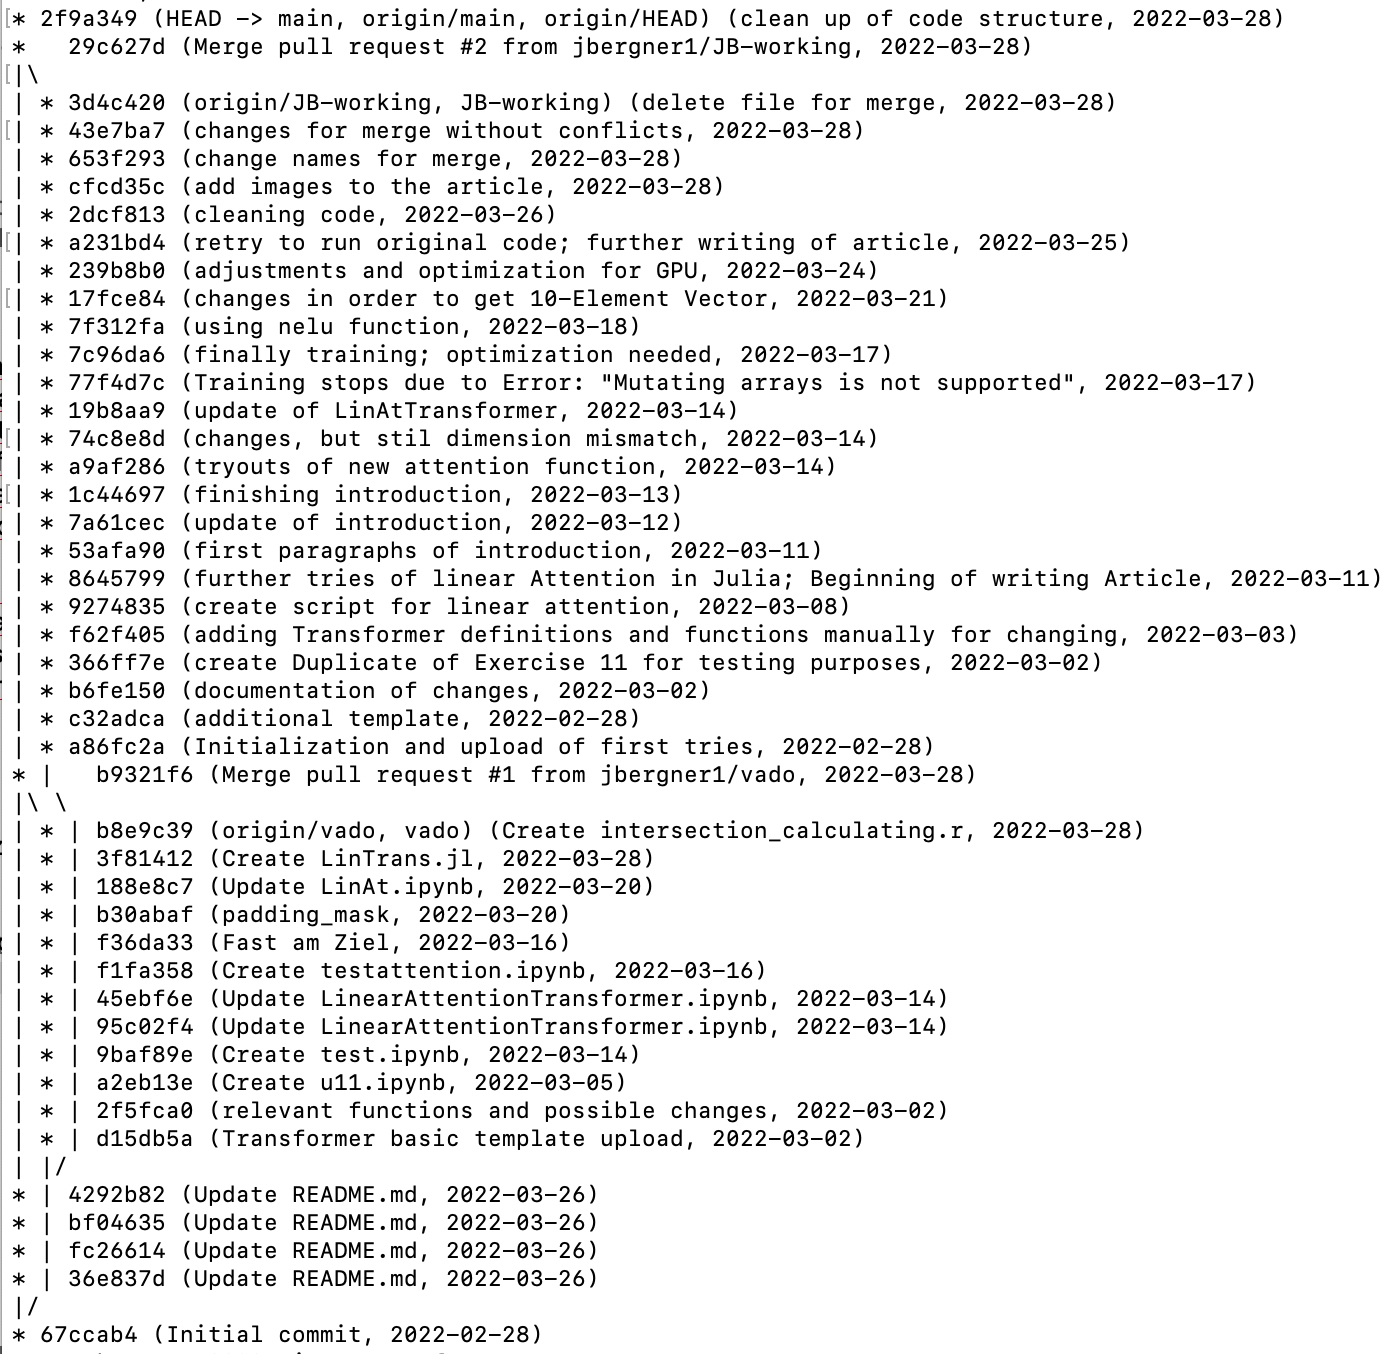
\includegraphics[width=\textwidth]{gitHistory}
    \label{fig:mesh1}
\end{figure}

\end{document}


